\chapter{Analysis}
As a part of the multi project, we are not directly solving the problem ourselves, but providing a part such that the other project groups can perform that task easier.
As we did not solve the problem directly we have made our own problem definition:
	\textit{How can we provide a set of tools which can help develop application for the GIRAF-system?}
As a way to solve this we have chosen to make 3 projects, a library providing methods and classes, a database to save information and an application to control the content of the database. 

\section{Requirements}
When we where to develop our library we asked the other groups to supply requirements. We received the following requirements:
Save data on the device
Various classes for:
Profiles
Media
Apps
Departments
From this we derived some features which will be shown in appendix FeatureList.

\section{System architecture}
\subsection{In the multi project}
The way Oasis fit into the multi project, is by being a middle layer between the Apps and the server, as seen in picture \vref{fig:bigPic}. Oasis will handle the communication from the apps to save in the local database, as well as synchronizing the local database, with the server.

\begin{figure}
	\centering
		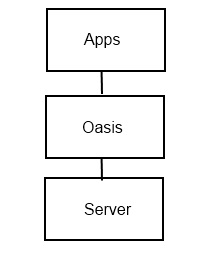
\includegraphics[width=\textwidth]{images/BigPicture.jpg}
	\caption{The multi project architecture}
	\label{fig:bigpic}
\end{figure}

\subsection{Each part}
Oasis consists of 3 parts, the oasis library which is the core of the project, the administration app, and the local database, as shown in picture \vref{fig:smallPic}. The Oasis library will handle applications interaction with the local database, and every giraf app should be utilizing this library. The Oasis library will also make sure that the local database is synchronized with the server's database.
The administration application is an app from which the user can interact with the database directly, creating or deleting users and departments, and making sure these are connected.

\begin{figure}
	\centering
		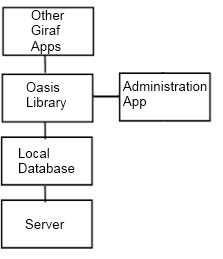
\includegraphics[width=\textwidth]{images/smallPicture.png}
	\caption{The project part architecture}
	\label{fig:smallpic}
\end{figure}